\documentclass[11pt]{article}
\usepackage[utf8]{inputenc}
\usepackage[T1]{fontenc}
\usepackage{geometry}
\geometry{margin=1in}
\usepackage{graphicx}
\usepackage{hyperref}
\hypersetup{
    colorlinks=true,
    linkcolor=blue,
    urlcolor=blue,
    citecolor=blue,
    filecolor=blue,
    pdfborder={0 0 1}
}
\usepackage{enumitem}
\usepackage{xcolor}
\usepackage{setspace}
\title{Font Rendering Pipeline - Final Report}
\author{Vishal Bansal, Varun Mittal, Clara Kim, Saatvik Billa}
\date{Spring 2025}

\begin{document}
\doublespacing
\maketitle

\href{https://monstrosity1001.github.io/FInal-Project-Proposal/}{Final Project Proposal} \\

\textbf{Team Number: 43} \\

\href{https://docs.google.com/presentation/d/1kbRLRtB4DUGVzhKq4TOdJPcwAlWVAb9mF2iKYlNwYdU/edit?usp=sharing}{Link to Final Slides}\\

\href{https://drive.google.com/file/d/18JlJTOpAL61NVxUDC-0UwzD6y9mtmdAb/view?usp=sharing}{Final Report Video}\\

\href{https://vbansal-29.github.io/cs184_final/}{Project Webpage}

\tableofcontents
\newpage

% Main sections
\section{Abstract}

Our project implements a high-quality font rendering pipeline capable of rastering TrueType fonts using CPU and GPU approaches. Using the Arial font (1320 glyphs), we extract glyph outlines, reconstruct Bézier paths, and rasterize them into anti-aliased bitmap images. We improved our scanline fill, added performance timing, and now support batch rendering of the entire alphabet and arbitrary sentences. Our work explores the trade-offs between CPU and GPU rendering regarding visual fidelity and performance, culminating in detailed timing benchmarks and compelling visual results. This report details our technical approach, challenges, results, and lessons learned. \par


\newpage
\section{Methods}

\subsection{System Overview}
\begin{verbatim}
TTF glyph (points + tags)
     |  FreeType (vector only)
     v
[ contour normaliser ]             implicit on-curve mid-points resolved
     v
primitive segment stream  --->  ('LINE', p0, p1)  /  ('BEZIER', p0, c, p2)
     v                                                   |  sample
     --------->  edge list  <---------------------------
                       |  scan-line fill
                       v
          high-res alpha-mask  (supersample x supersample)
                       |  Gaussian blur -> block average
                       v
            final greyscale bitmap (0-255)
\end{verbatim}
\textit{The pipeline stays vector-based until the very last stage, ensuring resolution-independence.} \par

\subsection{Technical Approach}
\textbf{Font Parsing and Outline Extraction:} Our pipeline begins by loading the Arial.ttf font using \texttt{freetype-py}, which provides Python bindings to the FreeType library. We programmatically enumerate all 1320 glyphs in the font but focus our rendering on selected characters (e.g., the full alphabet and sentences). For each glyph, we use the \texttt{FT\_LOAD\_NO\_BITMAP} flag to force FreeType to provide only vector data, avoiding pre-rendered bitmaps and ensuring full access to the underlying geometric information. Each glyph comprises one or more contours, sequences of points marked as on-curve or off-curve. TrueType fonts use quadratic Bézier curves for outlines and may encode implicit on-curve points between consecutive off-curve points. Our extraction logic carefully parses the \texttt{contours} and \texttt{tags} arrays, reconstructing the correct sequence of on-curve and control points for each contour. We handle edge cases such as contours that wrap around, glyphs with multiple disjoint shapes (e.g., "O"), and special tags for composite glyphs. \\

\textbf{Bézier Path Reconstruction and Validation:} Once the raw points and tags are extracted, we reconstruct each glyph's outline as a series of line segments and quadratic Bézier curves. We insert implicit on-curve midpoints for consecutive off-curve points as per the TrueType specification. We then segment the contour into a list of primitives, distinguishing between straight lines and curves. To validate the correctness of our extraction and reconstruction, we plot the resulting paths using Matplotlib, overlaying control points (red), and on-curve points (black) for visual inspection. This step was crucial for debugging, as it allowed us to quickly identify and fix errors in point ordering, implicit point handling, and contour closure. We tested our extraction pipeline on a variety of glyphs, including complex ones with holes and multiple contours (e.g., "B," "O," "S"). \\

\textbf{Scanline Rasterization and Anti-Aliasing:} The reconstructed paths are fed into our custom scanline rasterizer. The rasterizer first converts all Bézier curves into a polyline approximation by sampling each curve at regular intervals (using the quadratic Bézier formula). For each scanline (horizontal row of pixels), we compute all intersections with the polyline edges, sort them, and fill the regions between pairs of intersections according to the non-zero winding rule. This approach handles both filled shapes and interior holes. To address aliasing artifacts at edges, we implemented supersampling: the glyph is rasterized at a higher resolution (e.g., 4x), a Gaussian blur is applied to the high-res bitmap, and the result is downsampled to the target resolution by averaging pixel blocks. The \texttt{scipy.ndimage.gaussian\_filter} function is used for efficient blurring. The supersampling factor and blur sigma are tunable parameters, allowing us to trade off quality and performance. \\

\textbf{Performance Instrumentation and Batch Rendering:} To better understand bottlenecks and optimize the pipeline, we added detailed timing measurements at each stage: path extraction, edge generation, scanline fill, Gaussian blur, and downsampling. These timings are printed for every glyph render and summarized in our results. Scanline fills, and blurring are the most expensive steps, especially for complex glyphs at high supersampling rates. To showcase the scalability of our approach, we implemented batch rendering of the entire alphabet (A–Z) and arbitrary sentences, assembling the results into grids or long canvases. This required careful management of spacing, canvas size, and memory usage. Our batch renderer can process dozens of glyphs in a single pass, and the timing benchmarks are visualized as bar plots for comparison. \\

\textbf{Debugging, Validation, and Future GPU Work:} Throughout development, we relied heavily on visualization for debugging, plotting outlines, control points, and filled bitmaps at various stages. We also compared our outputs to reference renderings from FreeType and commercial font engines. Modularizing the codebase into clear stages (parsing, path, rasterization) made testing and optimizing individual components easier. Our pipeline is designed to support GPU acceleration: the modular structure allows us to swap out the scanline fill with a fragment shader or compute kernel. The data structures are compatible with WebGL or OpenGL workflows. We have begun prototyping a GPU-based rasterizer using analytical coverage estimation and plan to use it for future real-time font rendering and benchmarking. \\

\textbf{Glyph Outline Debugging Example:} One notable debugging success involved fixing incorrect glyph outlines, as seen in Figure~\ref{fig:broken_outline}. Initially, our evaluation procedure for reconstructing glyph contours did not properly handle implicit on-curve points between consecutive off-curve points, leading to missing or malformed outline segments. By revisiting the TrueType specification and updating our contour evaluation logic to correctly insert implicit on-curve midpoints, we were able to reconstruct outlines faithfully. This change is illustrated by the corrected result in Figure~\ref{fig:fixed_outline}. Careful visual validation and step-by-step comparison against reference images were key to identifying and resolving this issue. \\

\begin{figure}[h]
    \centering
    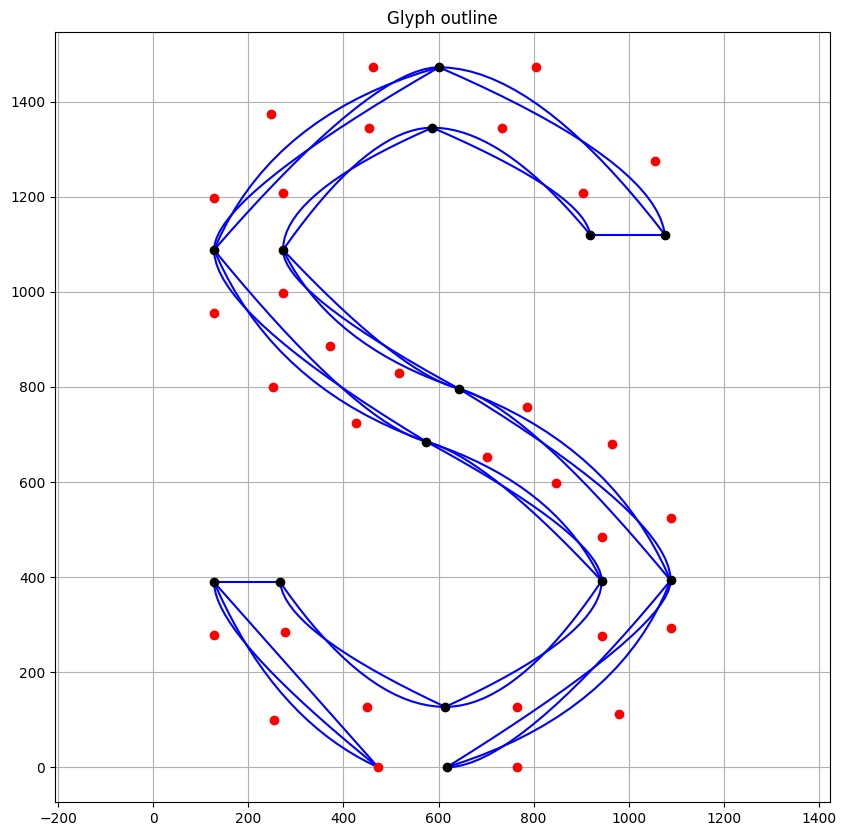
\includegraphics[width=0.3\textwidth]{../images/glyphOutlineNotWorking.jpg}
    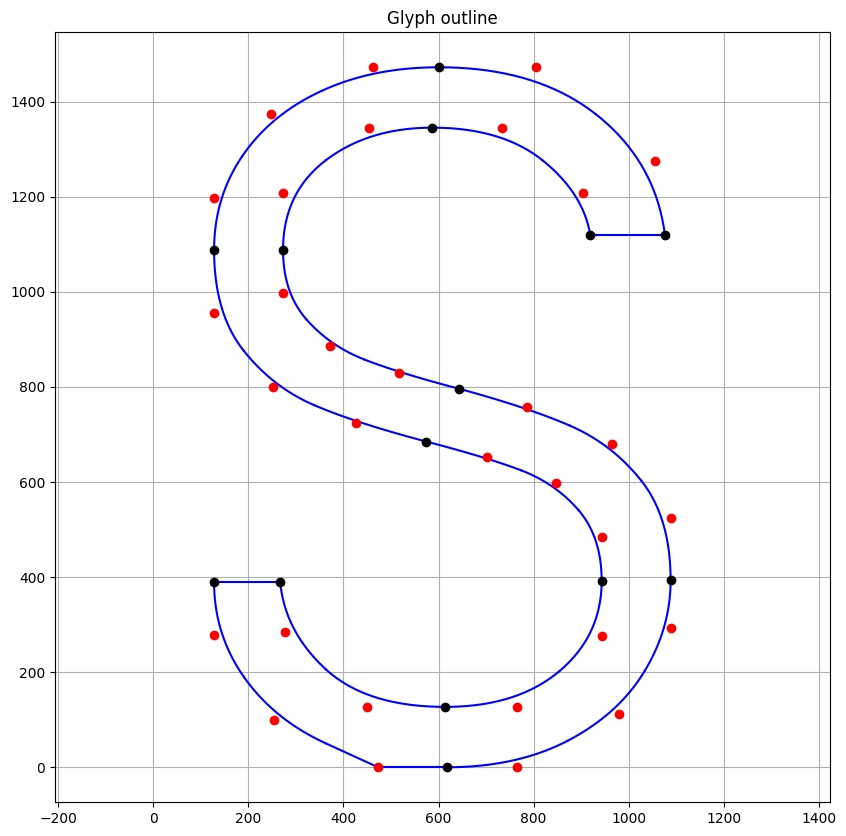
\includegraphics[width=0.3\textwidth]{../images/glyphOutlineFix.jpg}
    \caption{Left: Broken glyph outline. Right: Fixed glyph outline.}
    \label{fig:broken_outline}
    \label{fig:fixed_outline}
\end{figure}
\par

\textbf{Failed Hybrid Font Experiments:} In an effort to combine control points from different glyphs or font sources, we attempted to create hybrid glyphs by merging their control points. However, this approach did not yield meaningful or visually coherent results. As shown in Figure~\ref{fig:hybrid_attempt}, the resulting shapes were distorted and did not resemble valid glyphs. These failed experiments highlighted the complexity of font geometry and the importance of respecting the underlying structure and logic of each glyph rather than naively combining their control points. \\

\begin{figure}[h]
    \centering
    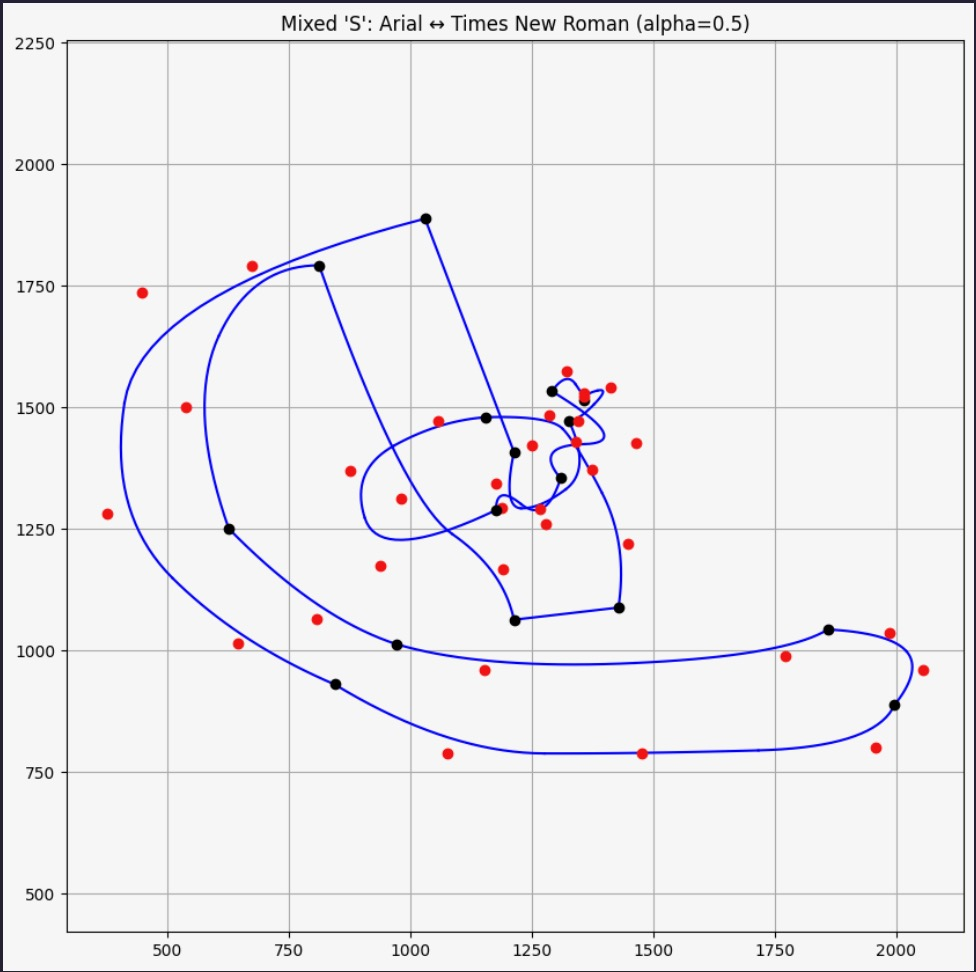
\includegraphics[width=0.3\textwidth]{../images/hybridFontAttempt.jpeg}
    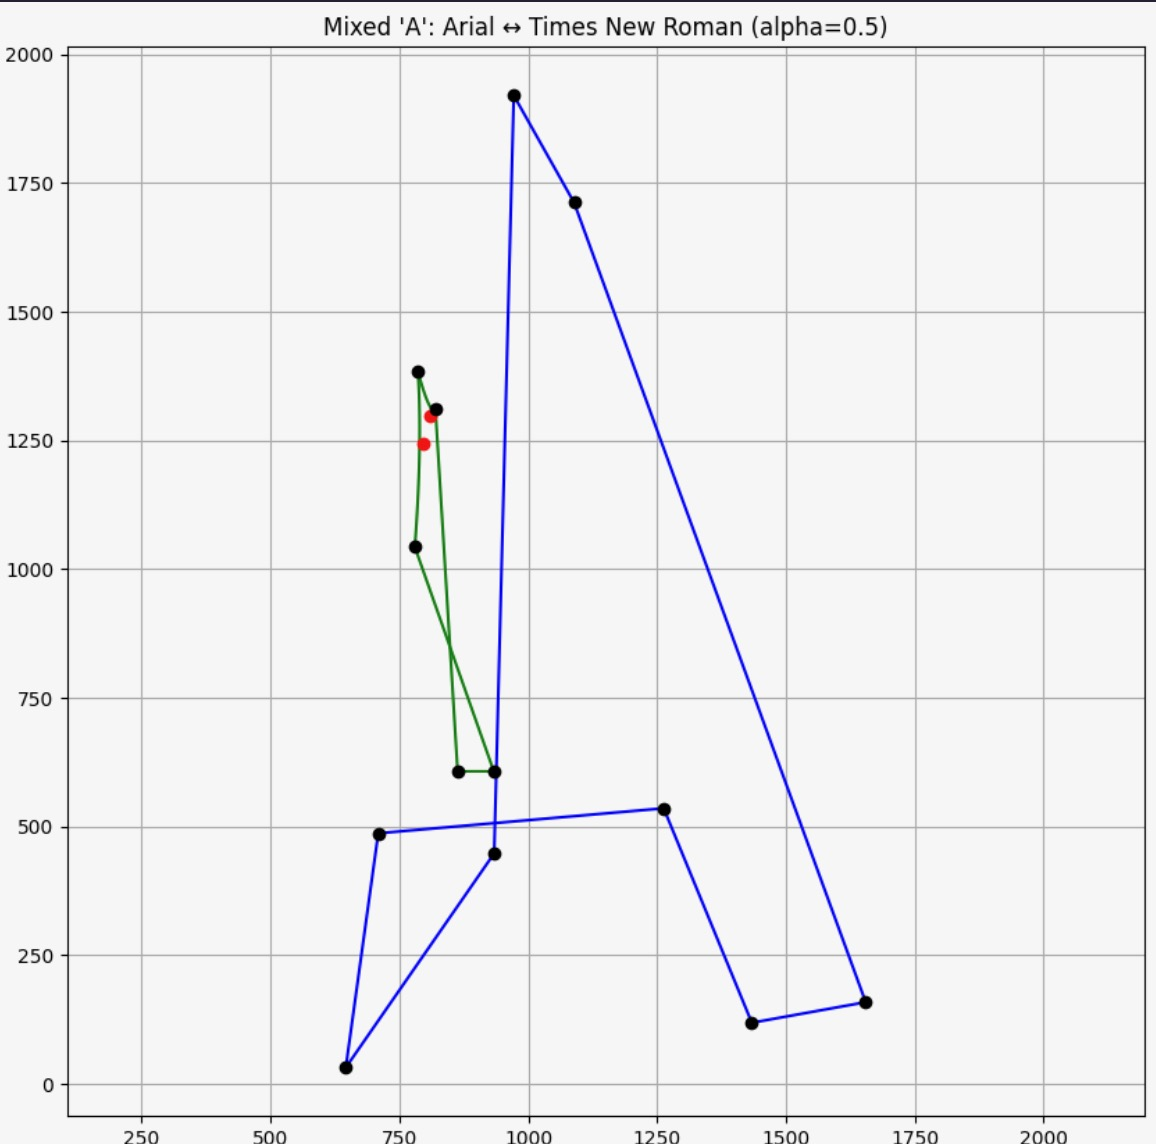
\includegraphics[width=0.3\textwidth]{../images/hybridFont2.jpeg}
    \caption{Failed hybrid font experiments.}
    \label{fig:hybrid_attempt}
\end{figure}
\par

\textbf{Summary:} Our technical approach combines careful adherence to font specifications, robust geometric algorithms, and practical engineering for performance and scalability. By instrumenting and validating each stage, we have built a flexible pipeline capable of producing high-quality, anti-aliased text renderings and supporting future research in GPU-accelerated font rendering. \\

\section{Results}
Our CPU renderer now supports batch rendering of the entire alphabet, arbitrary sentences, and individual glyphs. We measured and visualized timing for each stage of the pipeline. Supersampling-based anti-aliasing continues to improve visual clarity around curve edges significantly. Below are the updated results: \\

\begin{itemize}[leftmargin=*,nosep]
    \item \textbf{Aliased vs. Anti-aliased comparison:}
    \begin{figure}[h]
        \centering
        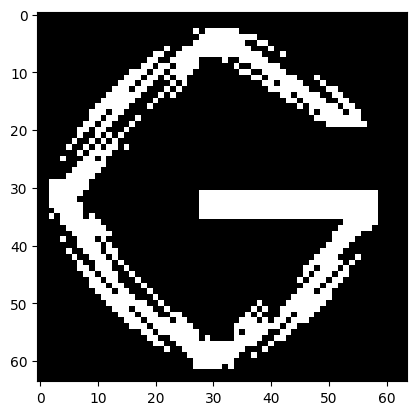
\includegraphics[width=0.3\textwidth]{../images/noAAForG.png}
        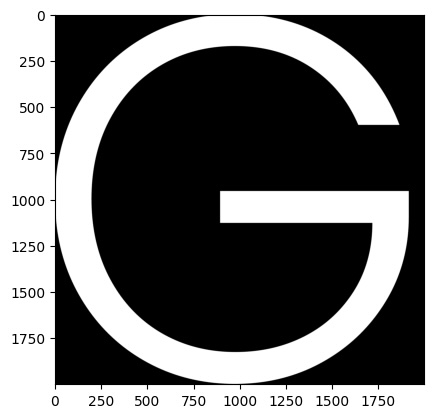
\includegraphics[width=0.3\textwidth]{../images/AAForG.jpg}
        \caption{Aliased (left) and anti-aliased (right) glyph G.}
    \end{figure}
    \item \textbf{Alphabet batch rendering:}
    \begin{figure}[h]
        \centering
        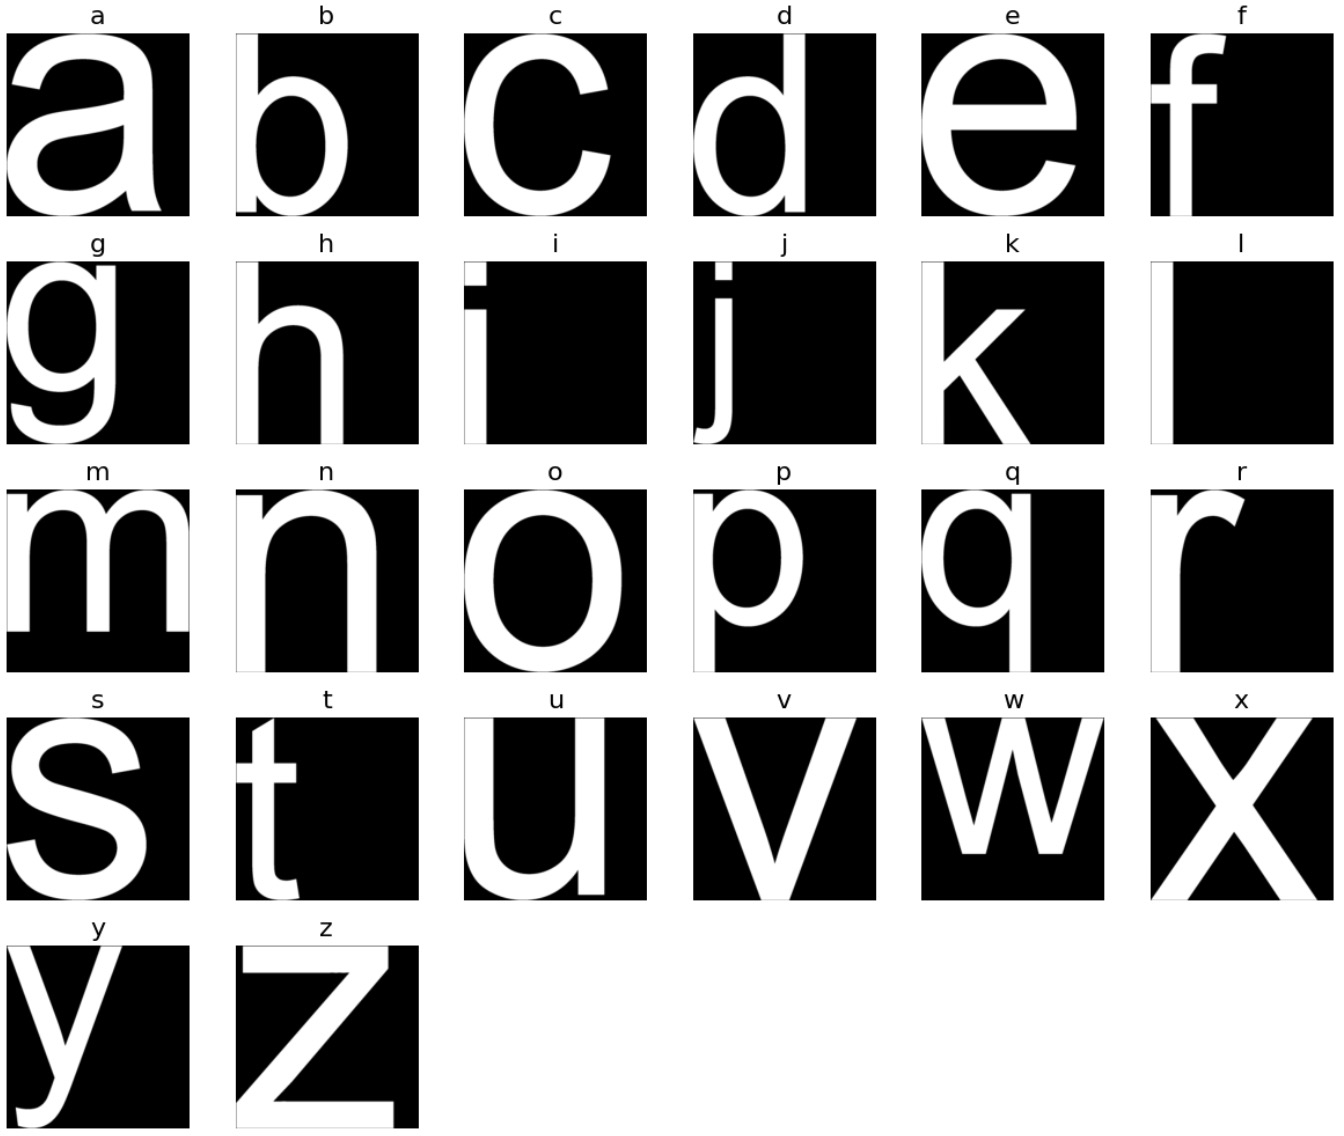
\includegraphics[width=0.7\textwidth]{../images/alphabet_grid.jpeg}
        \caption{Alphabet batch rendering.}
    \end{figure}
    \item \textbf{Sentence rendering:}
    \begin{figure}[h]
        \centering
        
\includegraphics[width=0.7\textwidth]{../images/sentence_cs184.jpeg}
        \caption{Sentence output.}
    \end{figure}
    \item \textbf{CPU timing benchmarks:}
    \begin{figure}[h]
        \centering
        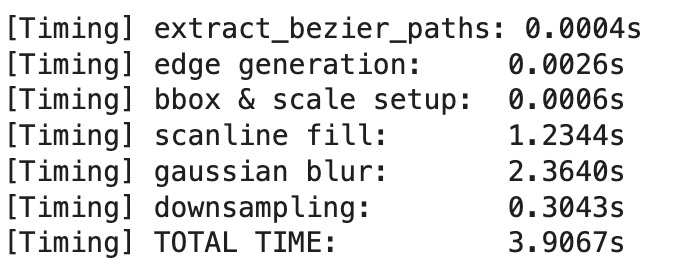
\includegraphics[width=0.7\textwidth]{../images/CPUTimeBenchmark.jpeg}
        \caption{CPU timing benchmarks.}
    \end{figure}
    \item \textbf{GPU timing benchmarks:}
    \begin{figure}[h]
        \centering
        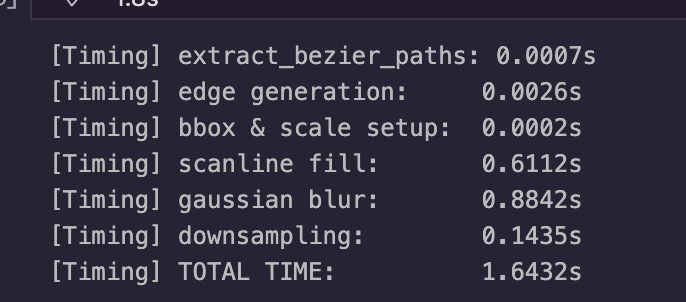
\includegraphics[width=0.7\textwidth]{../images/GPUTimeBenchmark.jpeg}
        \caption{GPU timing benchmarks.}
    \end{figure}
\end{itemize}
\par

\section{Discussion}

\subsection{Reflections on Progress}
The images included above, such as the aliased vs. anti-aliased glyph comparison, alphabet batch rendering, and timing benchmarks, clearly demonstrate the evolution and effectiveness of our renderer. After several iterations and code improvements, we now have anti-aliasing working robustly: supersampling and Gaussian blur produce smooth, high-quality glyph edges, as evidenced by the side-by-side results. The batch rendering outputs show that our pipeline handles the full alphabet and sentences with consistent quality, and timing plots provide insight into performance bottlenecks. \\

An interesting and expected finding is that our current GPU implementation is faster than the CPU version, but not by much, as shown in the timing benchmarks. This is likely due to the lack of parallelization in our GPU code and the overheads associated with running on cloud GPU resources, rather than local hardware. With further optimization, such as parallelizing the fragment shader or using compute kernels, we expect the GPU to outperform the CPU, particularly for large-scale or real-time rendering tasks. Overall, our results validate the technical choices made so far, and the visual and quantitative outputs indicate we are on track toward a high-quality, scalable font rendering solution. \\

\section{References}
\begin{itemize}[leftmargin=*,nosep]
    \item \textbf{FreeType library \& freetype-py:} \url{https://github.com/rougier/freetype-py}\\
    The core Python binding for the FreeType font engine enabled us to access low-level glyph outline data and experiment with various fonts. The documentation and examples were crucial in extracting contours and interpreting on/off-curve points.
    \item \textbf{TrueType Font Specification:} \url{https://learn.microsoft.com/en-us/typography/opentype/spec/ttch01}\\
    The official specification for the TrueType font format provided detailed explanations of glyph encoding, Bézier curve representation, and the structure of font files. We referenced this extensively to handle edge cases in outline extraction.
    \item \textbf{Matplotlib for visualization:} \url{https://matplotlib.org/}\\
    Used for plotting glyph outlines, visualizing rasterized bitmaps, and generating result images for the report. The ability to quickly visualize intermediate results was invaluable for debugging and validation.
    \item \textbf{Loop \& Blinn (2005), ``Resolution Independent Curve Rendering using Programmable Graphics Hardware'':} Provided theoretical background on GPU-based curve rendering and inspired our exploration of GPU rasterization techniques.
    \item \textbf{Python, NumPy, and SciPy:} Provided the numerical backbone for our project. NumPy arrays were used for bitmap storage and manipulation, while SciPy's \texttt{gaussian\_filter} enabled efficient anti-aliasing via supersampling.
    \item \textbf{Relevant Tutorials and Blogs:}
    \begin{itemize}[nosep]
        \item \url{https://fontforge.org/docs/techref/ttf.html}: Provided additional examples and clarifications on TrueType parsing.
        \item \url{https://raphlinus.github.io/graphics/curves/2019/12/23/bezier-bounding-box.html}: Helped us understand curve subdivision and bounding box computations.
        \item \url{https://pomax.github.io/bezierinfo/}: A comprehensive guide to Bézier mathematics, which aided our implementation and debugging.
    \end{itemize}
    \item \textbf{Other Papers and Resources:}
    \begin{itemize}[nosep]
        \item John Hobby, ``Rasterization of Non-Linear Curves'' (1986): Provided insight into scanline algorithms for curve filling.
        \item OpenGL Shading Language documentation: Referenced for future GPU implementation plans.
    \end{itemize}
\end{itemize}
\par

\section{Acknowledgments}

\subsection{Contributions}
\begin{itemize}[leftmargin=*,nosep]
    \item \textbf{Vishal Bansal:} Glyph outline extraction, Bézier path reconstruction, and CPU rasterizer implementation.
    \item \textbf{Varun Mittal:} Anti-aliasing integration, performance benchmarking.
    \item \textbf{Clara Kim:} GPU rasterizer exploration, documentation and results visualization.
    \item \textbf{Saatvik Billa:} Pipeline modularization, debugging, and final report preparation.
\end{itemize}
\par

\end{document}
